\documentclass[10pt, a4paper]{article}

% On écrit en français
\usepackage[utf8]{inputenc}
\usepackage[frenchb]{babel}
\usepackage[T1]{fontenc}

% Packages nécessaires
\usepackage{graphicx}
\usepackage{hyperref}
\usepackage{eurosym}
\usepackage{wrapfig}
\usepackage{lscape}
\usepackage{minted}

% Diagrammes de séquences
\usepackage{tikz}
\usetikzlibrary{arrows, shadows}
\usepgflibrary{arrows}
\usepackage[underline=true, rounded corners=false]{pgf-umlsd}

% Document "fancy"
\usepackage{fancyhdr}
\pagestyle{fancy}
\fancyhf{}

% Gros en-têtes/pied de pages
\renewcommand{\headrulewidth}{2pt}
\renewcommand{\footrulewidth}{1pt}

% Police Helvetica <3
\usepackage{helvet}
\renewcommand*{\familydefault}{\sfdefault}

% Enlever les alinéas
\setlength{\parindent}{0pt}

% Sous titre de document
\usepackage{titling}
\newcommand{\subtitle}[1]{%
  \posttitle{%
    \par\end{center}
    \begin{center}\large#1\end{center}
    \vskip0.5em}%
}

% Nom du projet
\def \DocumentTitle {TP Algorithme expérimentale}

% Contenu des en-têtes/pied de pages
\fancyhead[RE,LO]{\DocumentTitle}
\fancyfoot[CE,CO]{\leftmark}
\fancyfoot[LE,RO]{\thepage}

\begin{document}

% En tête complet de document
\title{\DocumentTitle}
\author{
    TURPIN Pierre
}
\date{\today}
\maketitle \newpage
\tableofcontents \newpage

\section{Mesure du temps d'exécution du programme}

\subsection{Découverte de l'aspect stochastique du programme}

La compilation de la source est faite en mode débug avec l'option -g de gcc. \\

\begin{minted}{bash}
gcc -g -o ./markov ./markov.c
\end{minted}

Les options d'exécutions du programme seront k = 3 et m = 1 000 000 en
utilisant le fichier texte \emph{don-quixote.txt}. \\

L'éxécution avec ces paramètres est lancées 3 fois. \\
Les temps d'exécution de celle-ci sont mesurés par la command \emph{time} et
sont enregistrés dans le même fichier. \\
Les résultats d'exécution sont également stockés dans des fichiers différents. \\


\begin{minted}{bash}
rm -f ./t

/usr/bin/time -a -o ./t -f "%e" ./markov 3 1000000 < ./don-quixote.txt > ./tmp1
/usr/bin/time -a -o ./t -f "%e" ./markov 3 1000000 < ./don-quixote.txt > ./tmp2
/usr/bin/time -a -o ./t -f "%e" ./markov 3 1000000 < ./don-quixote.txt > ./tmp3
\end{minted}

Dans le fichier de temps d'exécution, on remarque que les trois lignes
diffèrent. Cela signifie que la durée de chaque exécution est différentes. \\

Les fichiers de résultats contiennent chacun des textes complètement différent. \\

Ces différences doivent être du à une instruction stochastique dans le programme. \\

\subsection{Mesure du temps d'exécution avec k=3, m=1000000}

Le programme est lancé 100 fois avec les même paramètres avec les fichiers
d'entrées \emph{don-quixote.txt}, \emph{madame-bovary.txt} et \emph{zadig.txt}.
Les résultats sont ignorés dans cette étude. Seul les temps d'exécutions sont
enregistrés dans un fichier par texte. \\

\begin{minted}{bash}
# Nettoyage des fichiers de temps d'execution
rm -f ./tD
rm -f ./tM
rm -f ./tZ

for i in $(seq 1 100); do
  /usr/bin/time -a -o ./tD -f "%e" ./markov 3 1000000 < ./don-quixote.txt > /dev/null
done

for i in $(seq 1 100); do
  /usr/bin/time -a -o ./tM -f "%e" ./markov 3 1000000 < ./madame-bovary.txt > /dev/null
done

for i in $(seq 1 100); do
  /usr/bin/time -a -o ./tZ -f "%e" ./markov 3 1000000 < ./zadig.txt > /dev/null
done
\end{minted}

Les temps d'exécution sont visible sur l'histogramme
\ref{fig:chart_k3_m1000000}. Le texte de Don Quixote prend beaucoup plus de
temps que les autres. \\
On voit pour chaque texte que le temps de l'exécution est différentes à chaque
lancement. Cela montre l'aspect stochastique du programme. \\

\begin{figure}[ht]
    \centering
    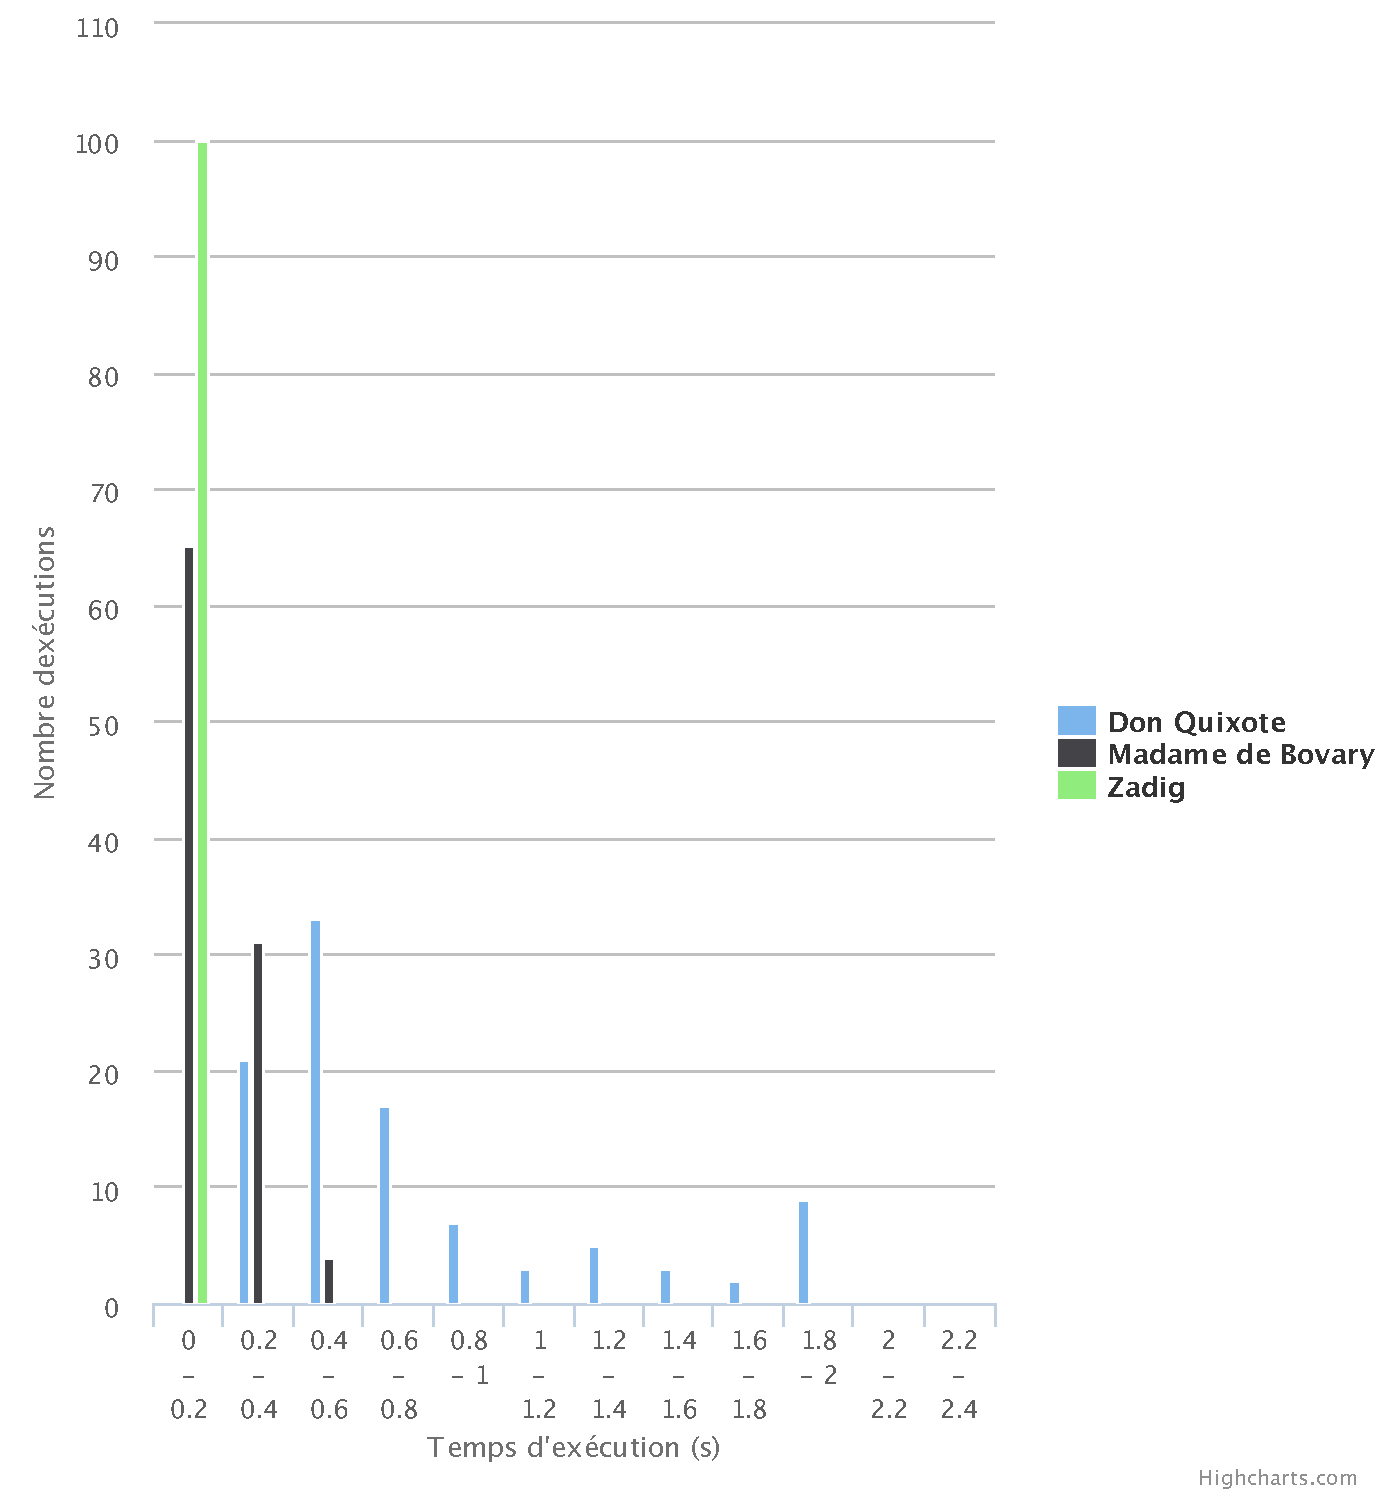
\includegraphics[width=1.0\textwidth]{chart_k3_m1000000}
    \caption{Temps d'exécution du programme avec k=3 et m=1000000}
    \label{fig:chart_k3_m1000000}
\end{figure}

\subsection{Suppression de l'aspect stochastique}

Le programme utilise la fonction \emph{rand} de la bibliothèque C. Cette
fonction est une interface au générateur de nombre pseudo aléatoire de la
bibliothèque. Ce générateur s'initialise par une \emph{seed} avec la fonction
d'API \emph{srand}. \\

Pour supprimer l'aspect aléatoire du programme, l'appel à \emph{srand} dans le
code est commenté. \\

Plusieurs exécutions avec les même paramètres rendent exactement le même
résultat et ont un temps d'exécution très semblable (< à 2ms de différences). \\

\subsection{Influence de la charge CPU}

Pour vérifier si la charge du CPU influe sur le temps d'exécution, 20
exécutions pour chaque texte sont lancées en parallèles. On s'attend alors à
voir que ceux utilisant le texte de Zadig sont ralenties par les autres
exécutions. \\

\begin{minted}{bash}
# Nettoyage des fichiers de temps d'execution
rm -f ./tDC
rm -f ./tMC
rm -f ./tZC

for i in $(seq 1 20); do
  /usr/bin/time -a -o ./tDC -f "%e" ./markov 3 1000000 < ./don-quixote.txt > /dev/null &
done
for i in $(seq 1 20); do
  /usr/bin/time -a -o ./tMC -f "%e" ./markov 3 1000000 < ./madame-bovary.txt > /dev/null &
done
for i in $(seq 1 20); do
  /usr/bin/time -a -o ./tZC -f "%e" ./markov 3 1000000 < ./zadig.txt > /dev/null &
done
\end{minted}

Les temps d'exécution sont visible sur l'histogramme
\ref{fig:chart_k3_m1000000_para}. Les temps d'exécution sont clairement
ralenties par rapport à la première étude. Cela est du à la prise de CPU par
chacune des instances du programme. \\

\begin{figure}[ht]
    \centering
    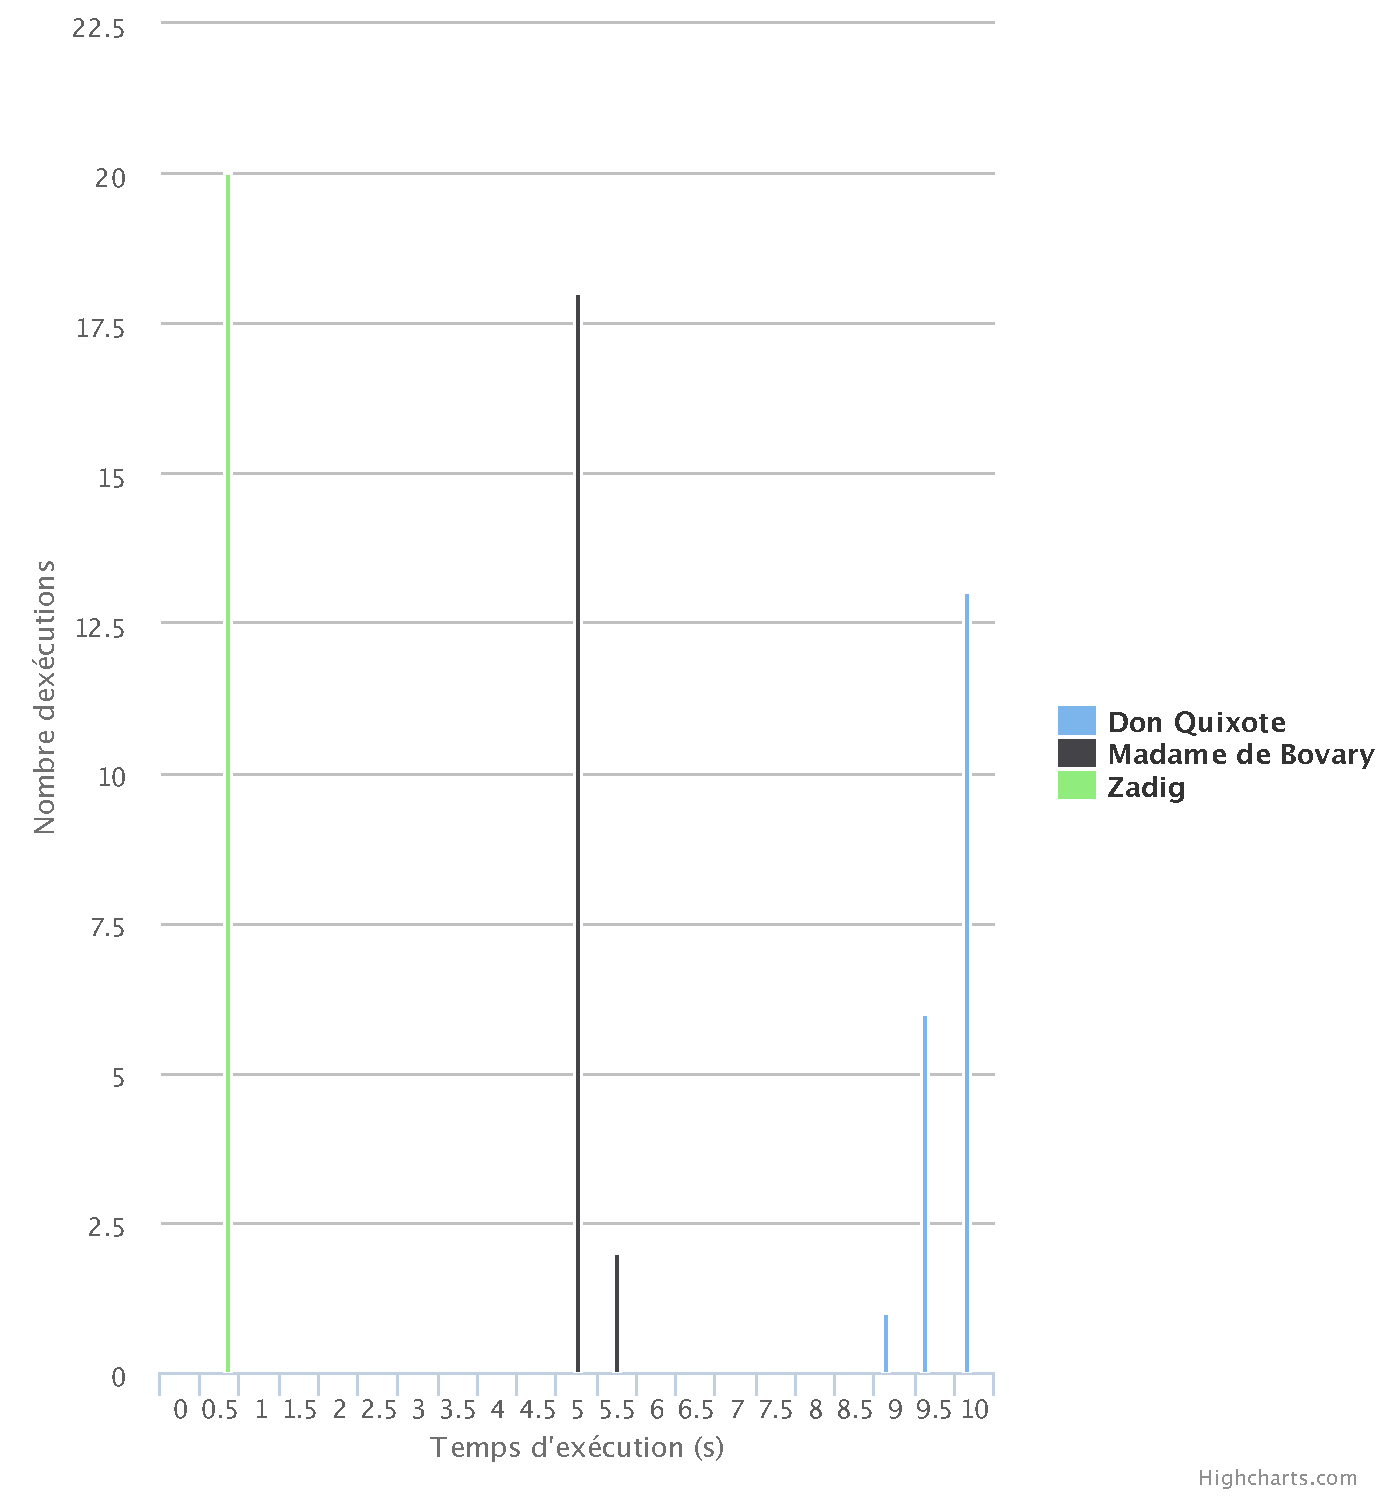
\includegraphics[width=1.0\textwidth]{chart_k3_m1000000_para}
    \caption{Temps d'exécution du programme avec k=3 et m=1000000 avec toute les exécutions en parallèles}
    \label{fig:chart_k3_m1000000_para}
\end{figure}

\subsection{Optimisation par le compilateur}

Le programme est recompilé en mode release optimisé en utilisant l'option
\emph{-O3} de \emph{gcc} :

\begin{minted}{bash}
gcc -O3 -o ./markov ./markov.c
\end{minted}

L'étude du temps d'exécution est à nouveau effectué seulement sur le fichier de
Don Quixote. Les 100 exécutions ne seront pas lancées en parallèles. \\

\begin{minted}{bash}
# Nettoyage des fichiers de temps d'execution
rm -f ./tO3

for i in $(seq 1 100); do
  /usr/bin/time -a -o ./tO3 -f "%e" ./markov 3 1000000 < ./don-quixote.txt > /dev/null
done
\end{minted}

Les temps sont comparés à ceux des exécutions sans le paramètre d'optimisation.
Le graphique \ref{fig:chart_k3_m1000000_o3} montre bien que l'optimisation
accélère l'exécution du programme. \\

\begin{figure}[ht]
    \centering
    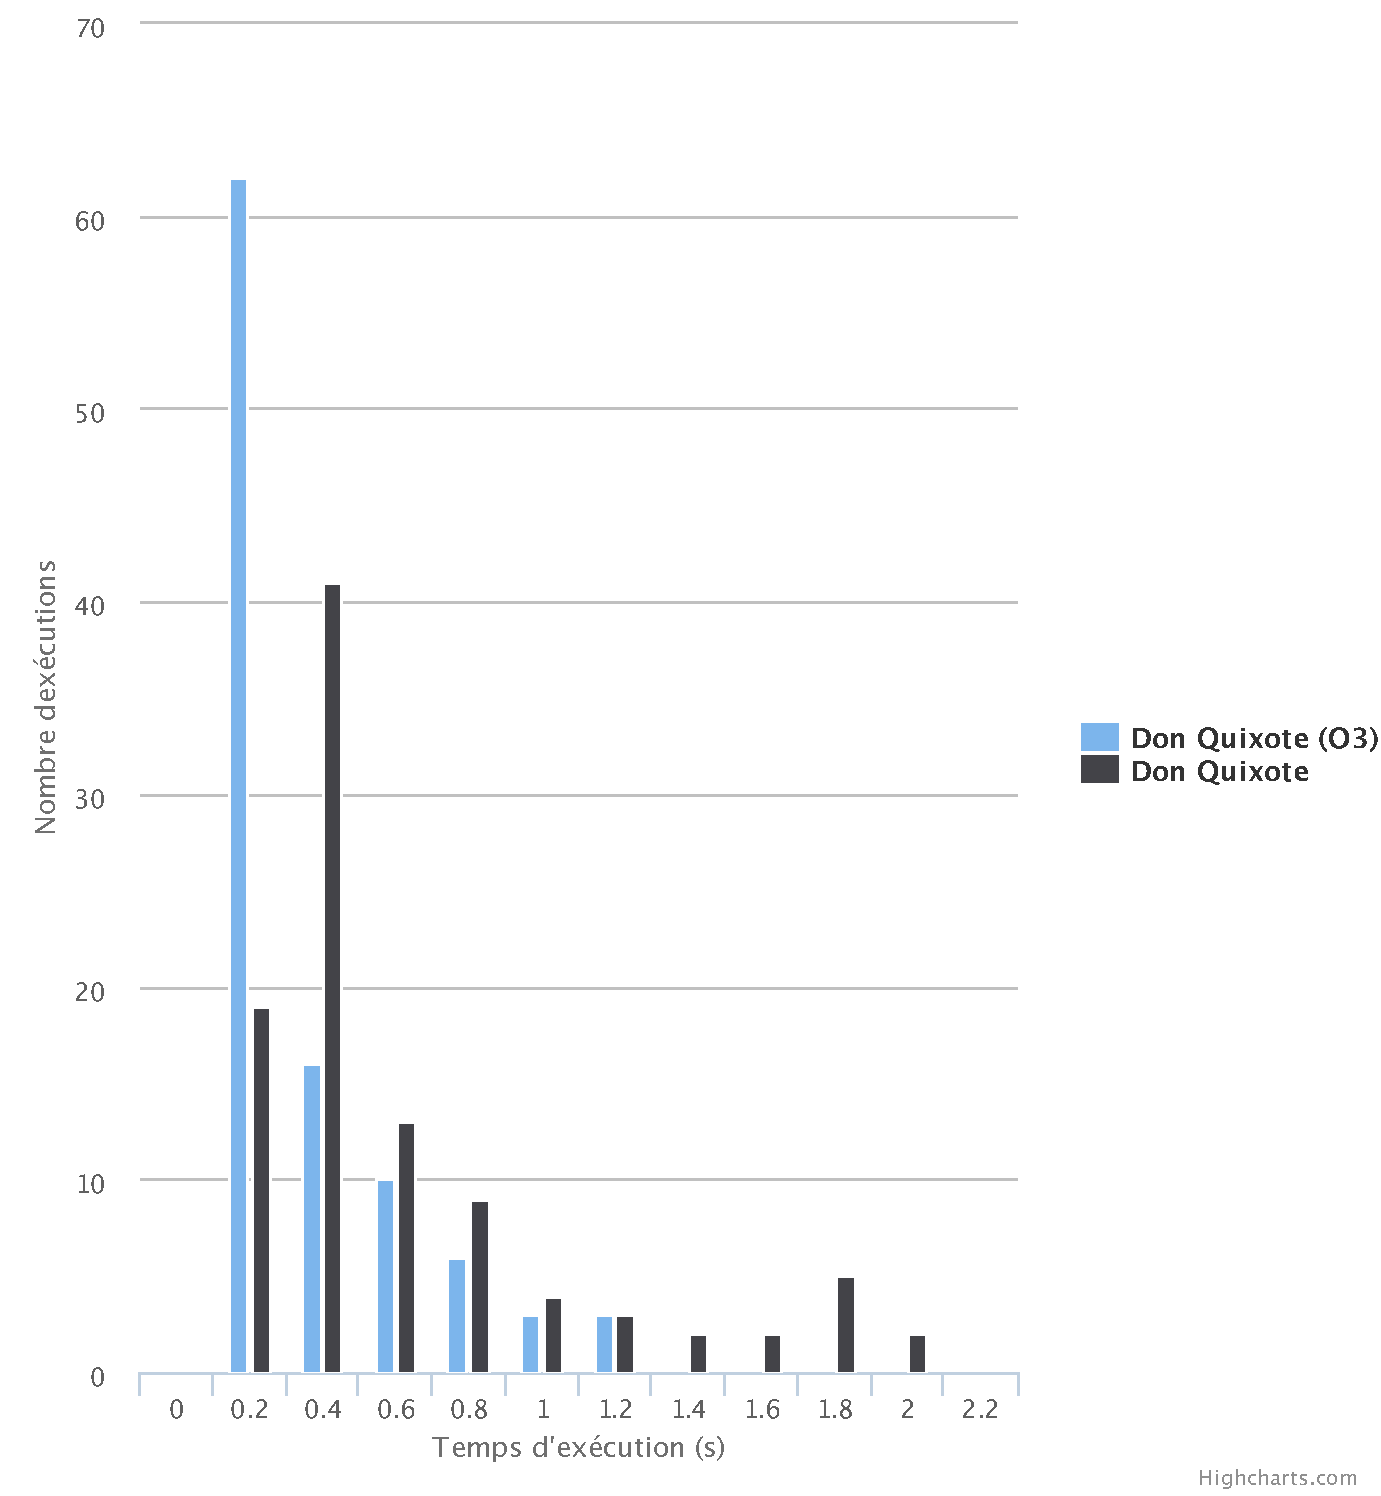
\includegraphics[width=1.0\textwidth]{chart_k3_m1000000_o3}
    \caption{Comparaison des temps d'exécution du programme avec k=3 et m=1000000 avec optimisation et sans}
    \label{fig:chart_k3_m1000000_o3}
\end{figure}

On obtient un temps médian de $0.34s$ avec l'optimisation et $0.54s$ sans. Le
pourcentage d'amélioration est donc de l'ordre de $37\%$

\section{Trouver l'opération dominante}

Pour trouver l'opération dominante, le programme est recompilé en mode débug
avec l'option \emph{-pg}. \\

L'exécutable est lancé une fois avec des paramètres fixes puis l'exécution peut
être analysé grâce au fichier \emph{gmon.out} avec le programme \emph{gprof}. \\

\begin{minted}{bash}
gcc -pg -o markov ./markov.c
./markov 3 1000000 < ./don-quixote.txt > /dev/null
gprof ./markov ./gmon.out
\end{minted}

Le résultat de \emph{gprof} est visible ci-dessous : \\

\begin{minted}{bash}
Flat profile:

Each sample counts as 0.01 seconds.
  %   cumulative   self              self     total           
 time   seconds   seconds    calls  ns/call  ns/call  name    
 65.97      0.32     0.32 10653342    29.72    29.72  wordncmp
 18.85      0.41     0.09                             main
  4.19      0.43     0.02   472367    42.56    42.56  skip
  3.14      0.44     0.02                             sortcmp
  0.00      0.44     0.00   157455     0.00     0.00  writeword
\end{minted}

La fonction la plus appelée dans le programme et qui prend le plus de temps
d'exécution est incontestablement \emph{wordncmp}. \\
Elle prend $65.97\%$ du temps d'exécution du programme. \\

L'exécution a été faite plusieurs fois pour pouvoir vérifier qu'on obtient le
même résultat malgré l'aspect stochastique du programme. \\

\section{Compter le nombre d'appels de l'opération dominante}

La fonction \emph{wordncmp} est utilisé dans trois buts : \\
\begin{itemize}
  \item initialisation du tableau word
  \item recherche dichotomique des préfixes candidats dans le tableau
  \item choix aléatoire d'un préfixe parmi les préfixes candidats
\end{itemize}
~\\

Chacune des utilisations est profilé en plaçant dans le code trois compteurs.
Ces trois compteurs sont ensuites affichés séparés par des espaces sur une
ligne de \emph{stderr}. \\

On remarque que l'exécution rend des résultats différents. Le programme est
lancé 100 fois avec comme paramètres ($k=3$, $m=1000000$,
text=./don-quixote.txt) pour pouvoir récupérer les valeurs médiannes. \\

\begin{minted}{bash}
# Nettoyage des fichiers de comptage
rm -f ./count

for i in $(seq 1 100); do
  ./markov 3 1000000 < ./don-quixote.txt > /dev/null 2>> ./count
done
\end{minted}

Les résultats donnent : \\
\begin{description}
  \item[7024519 appels médians] pour l'initialisation du tableau word
  \item[5243404 appels médians] pour la recherche dichotomique des préfixes
    candidats dans le tableau
  \item[936562 appels médians] pour le choix aléatoire d'un préfixe parmi les
    préfixes candidats
\end{description}
~\\

On remarque que l'initialisation du tableau word n'est pas atteint par l'aspect
stochastique. Le nombre d'appel à \emph{wordncmp} dans cette partie est donc
constant. \\

Au total, il y a $13204485$ appels médians pour la fonction \emph{wordncmp}. \\

\section{Mesurer la complexité de l'algorithme en fonction de n, m et k}

\subsection{Protocole expérimental}

Pour plus de rapidité de test, le programme est compilé avec l'option
d'optimisation \emph{-O3} du compilateur. \\

Dans cette étude, la variable \emph{count3} ainsi que le temps d'exécution sont
enregistrés. Pour voir l'évolution des résultats en fonction des variations des
trois variables $k, m, n$, plusieurs sous-études ont été menées. \\

Une sous-étude correspond à une configuration particulière. \\
Les trois textes sont utilisés donc $n\in\{404461, 112972, 26046\}$ pour,
respectivement, Don Quixote, Madame de Bovary et Zadig. \\
La variable $k$ est défini entre $2$ et $20$ inclus \footnote{Les temps
d'exécutions étaient trop grand pour k=1}\footnote{Sur certains graphiques, k=2
n'est pas montré car le temps d'exécution ou \emph{count3} étaient trop grand
ce qui rendait illisible les variations sur le reste du graphique.}. \\
La variable $m$ est testé entre $100000$ et $1000000$ avec un pas de $100000$. \\
Enfin comme chaque exécution est aléatoire, une sous-étude correspond à lancer
$100$ fois le programme avec la même configuration d'entrée. \\
Les valeurs résultantes de temps d'exécution et de \emph{count3} sont alors les
moyennes des $100$ exécutions. \\

Ce protocole d'exécution est effectué par ce script suivant : \\
\begin{minted}{bash}
#!/usr/bin/env sh

dir="./results"
rm -rf $dir
mkdir $dir

gcc -O3 -o ./markov ./markov.c

# Configuration de k
kMin=2
kMax=20
kStep=1

# Configuration de m
mMin=100000
mMax=1000000
mStep=100000

# Nombre d'exec par configuration
N=100

# Liste des textes
texts="don-quixote.txt madame-bovary.txt zadig.txt"

for txt in $texts; do
  n=$(cat $txt | wc -w)
  for k in $(seq $kMin $kStep $kMax); do
    for m in $(seq $mMin $mStep $mMax); do
      echo "$N executions avec k=$k, m=$m, n=$n, txt=$txt"
      for i in $(seq 1 $N); do
        /usr/bin/time -a -o "$dir/time-$txt-$k-$m-$n" -f "%e" \
          ./markov $k $m < $txt > /dev/null 2>> "$dir/count-$txt-$k-$m-$n"
      done
    done
  done
done
\end{minted}

Les résultats sont des simples fichiers contenants $100$ lignes chacun. Chaque
fichier est ensuite lu pour être moyenné puis structuré pour ensuite être
transformé en configuration de dataviz Highcharts.com (heatmap ou courbes)
\footnote{Les sources de ces transformations sont disponibles sur
\url{https://github.com/TurpIF/tp-markov-chain}}. \\

\subsection{Résultats et analyses}

Des heatmaps ont été générés avec $k$ variant sur les abscisses, $m$ sur les
ordonnées et la hauteur est soit le temps d'exécution, soit la valeur que prend
\emph{count3}.

\subsubsection{Temps d'exécution}

\begin{figure}[ht]
    \centering
    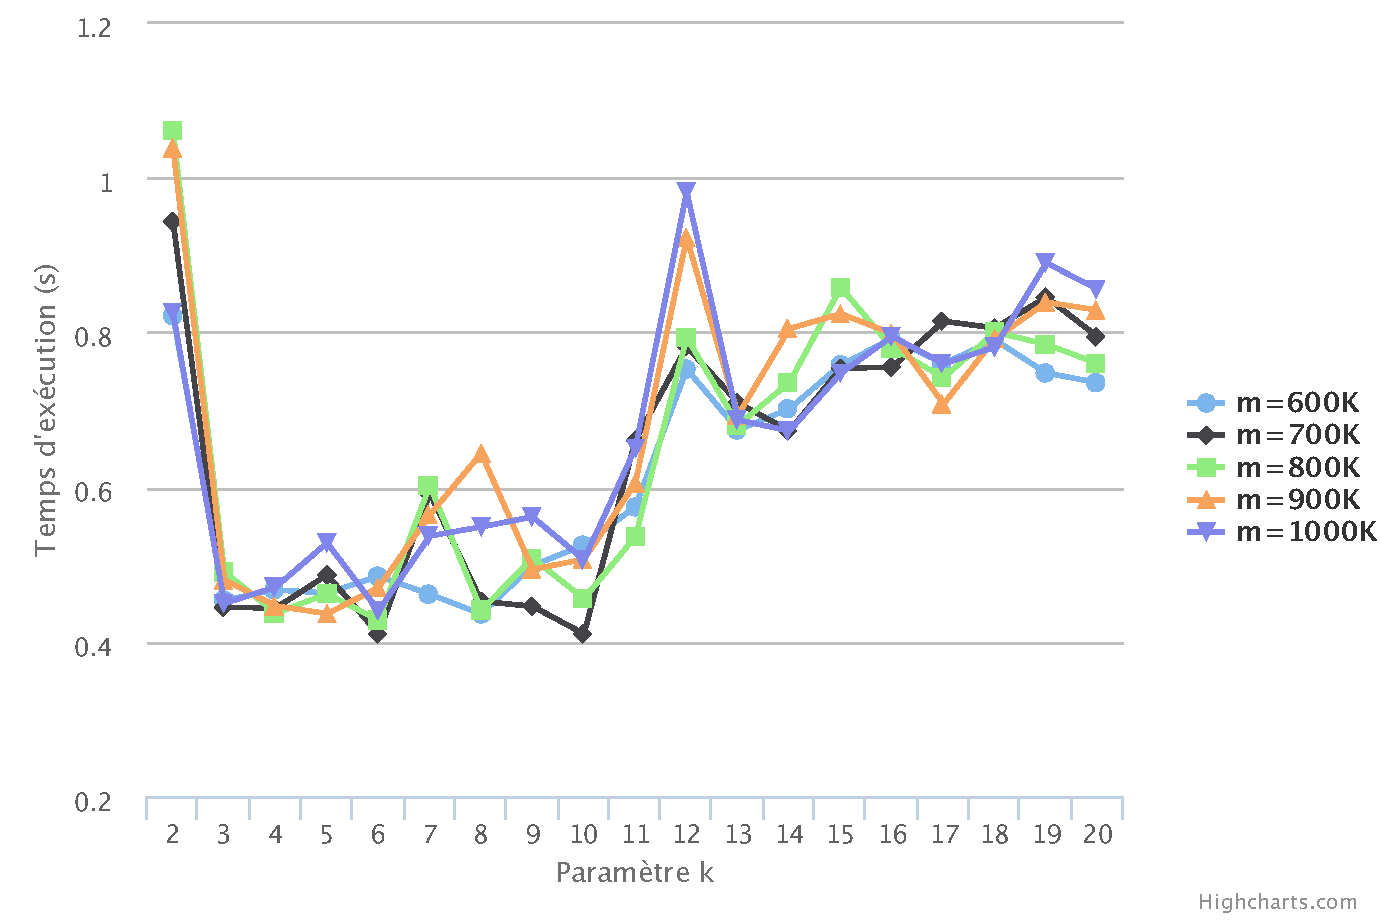
\includegraphics[width=1.0\textwidth]{time-don-quixote-plot}
    \caption{Temps d'exécution du programme en fonction de $k$ avec quelques $m$ donnés avec le texte de Don Quixote}
    \label{fig:time-don-quixote-plot}
\end{figure}

\begin{figure}[ht]
    \centering
    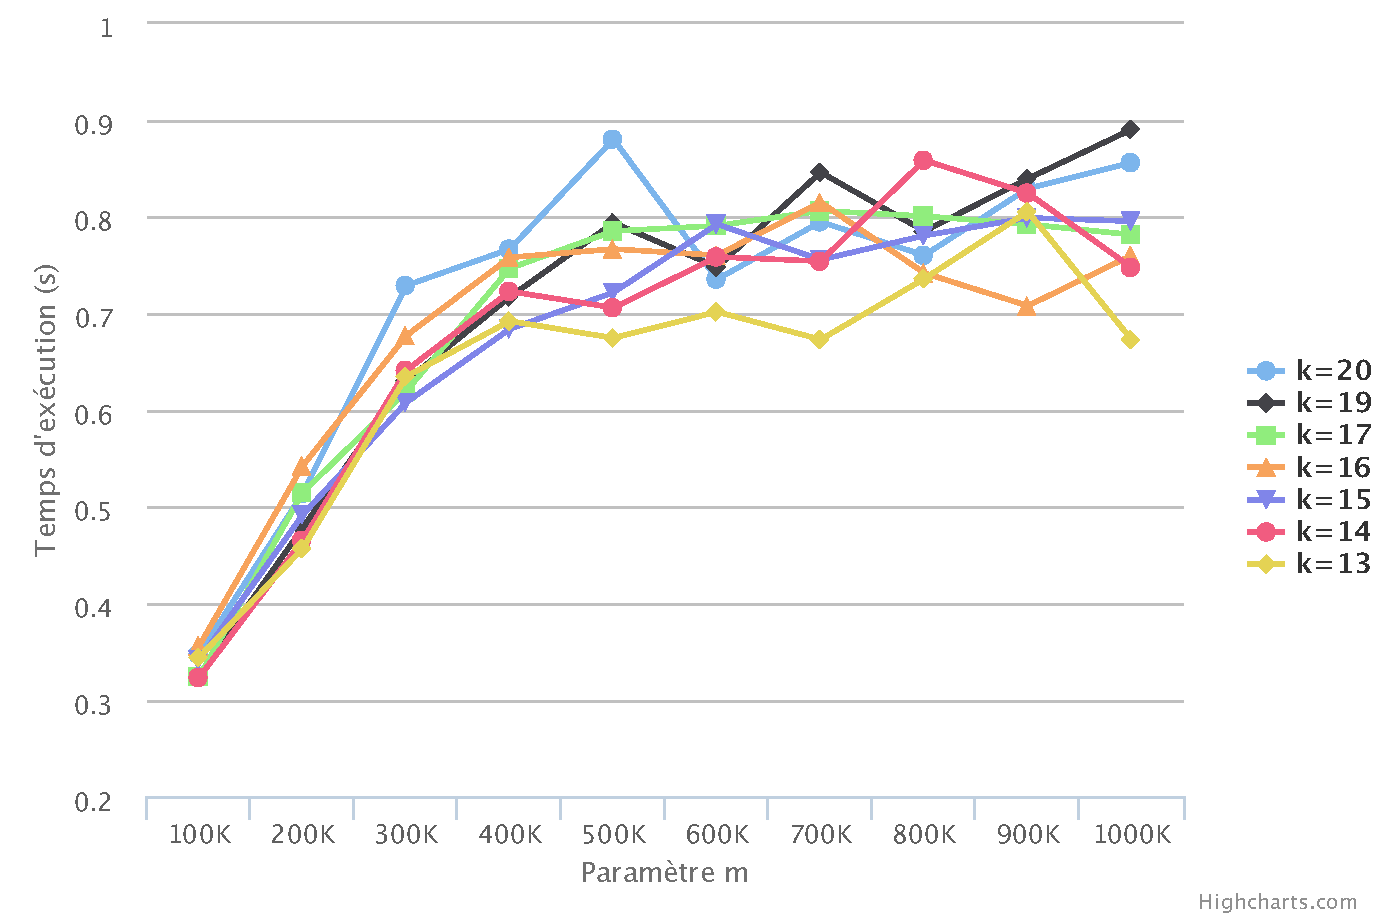
\includegraphics[width=1.0\textwidth]{time-don-quixote-plot-m}
    \caption{Temps d'exécution du programme en fonction de $m$ avec quelques $k$ donnés avec le texte de Don Quixote}
    \label{fig:time-don-quixote-plot-m}
\end{figure}

\begin{figure}[ht]
    \centering
    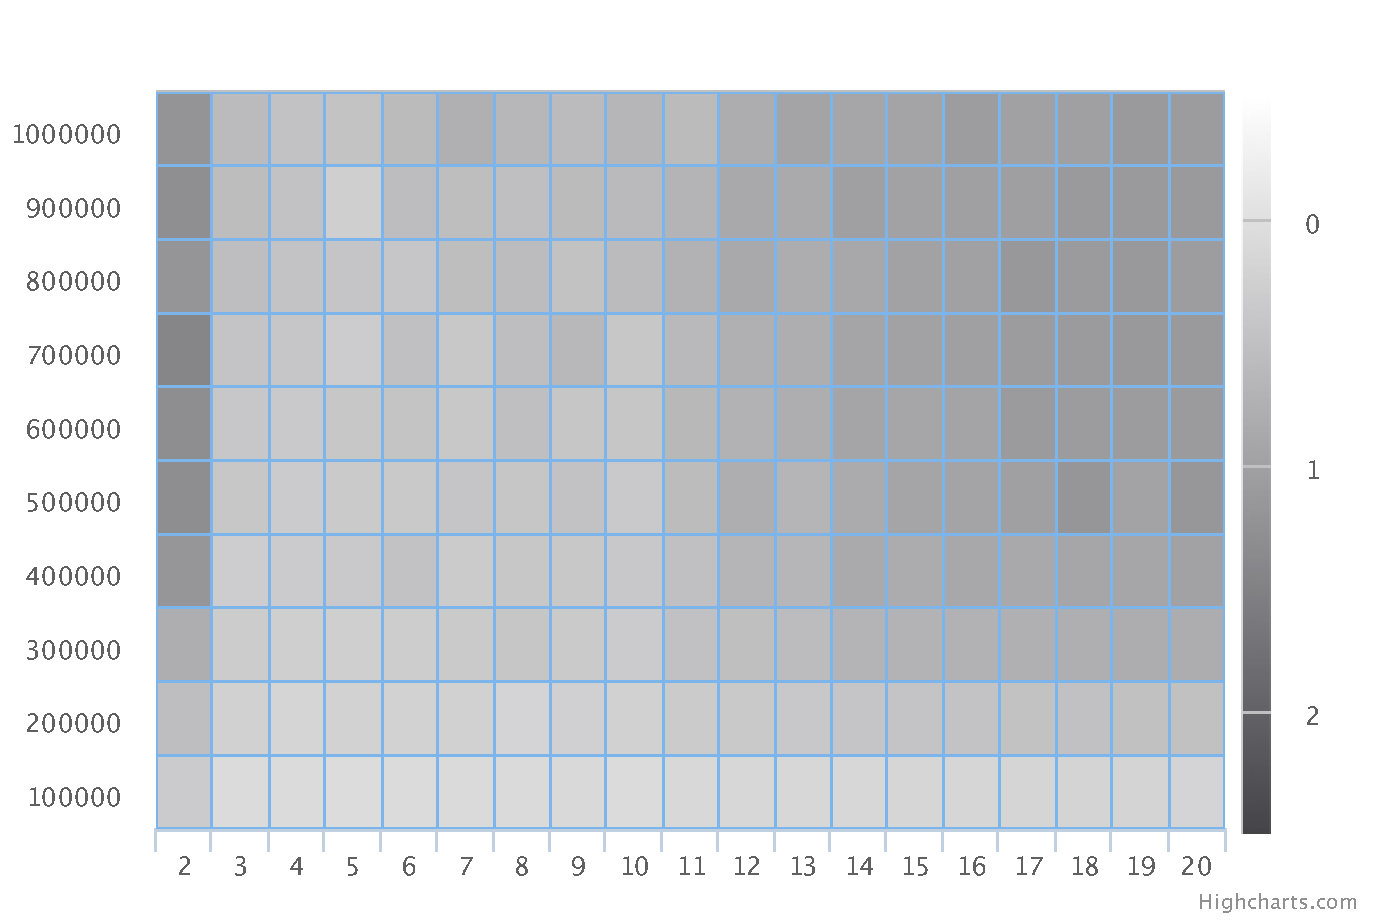
\includegraphics[width=1.0\textwidth]{time-don-quixote}
    \caption{Temps d'exécution du programme avec le texte de Don Quixote}
    \label{fig:time-don-quixote}
\end{figure}

\begin{figure}[ht]
    \centering
    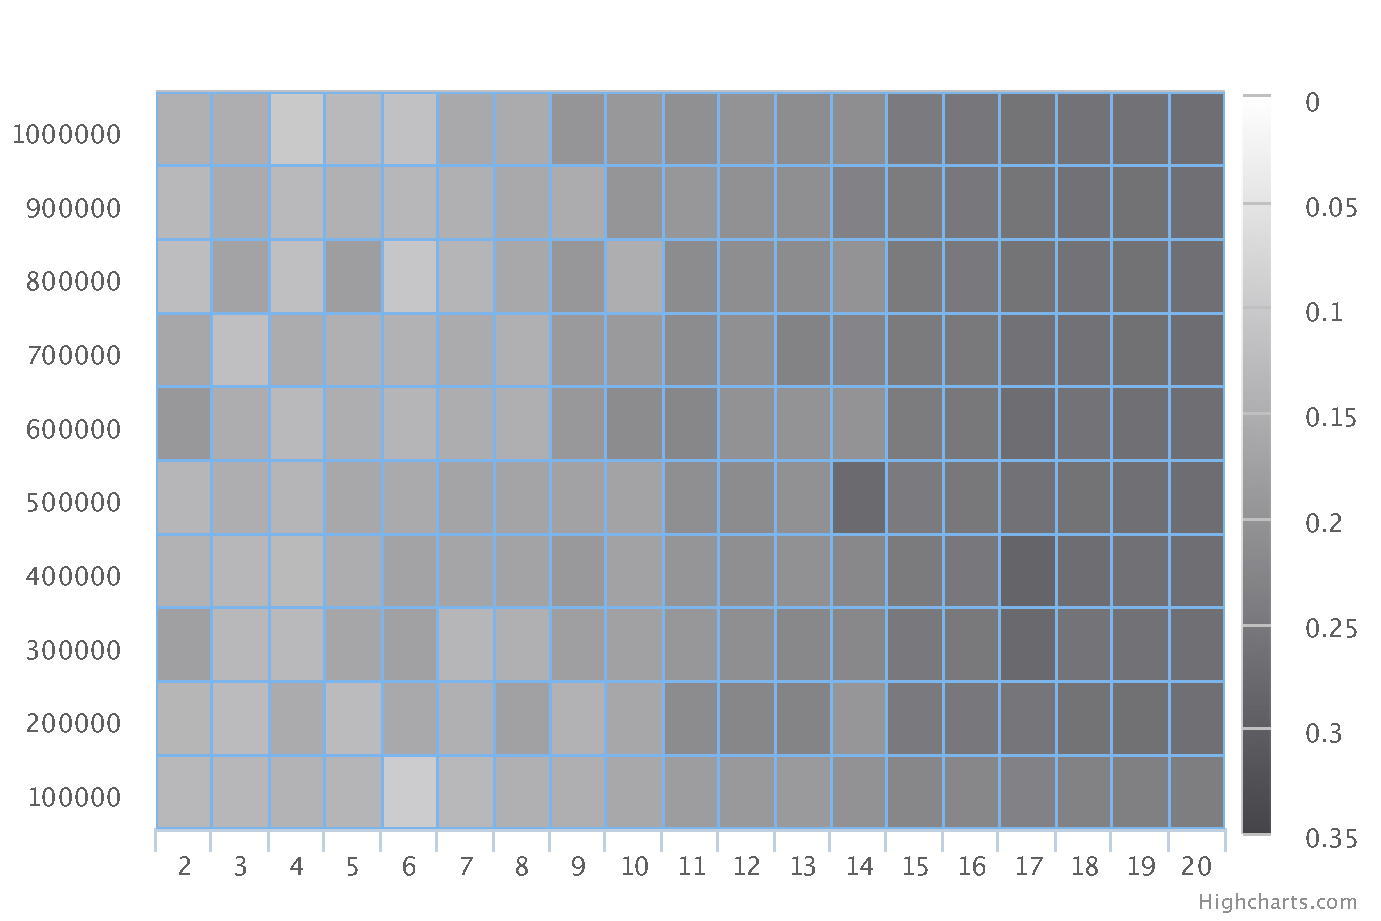
\includegraphics[width=1.0\textwidth]{time-madame}
    \caption{Temps d'exécution du programme avec le texte de Madame de Bovary}
    \label{fig:time-madame}
\end{figure}

\begin{figure}[ht]
    \centering
    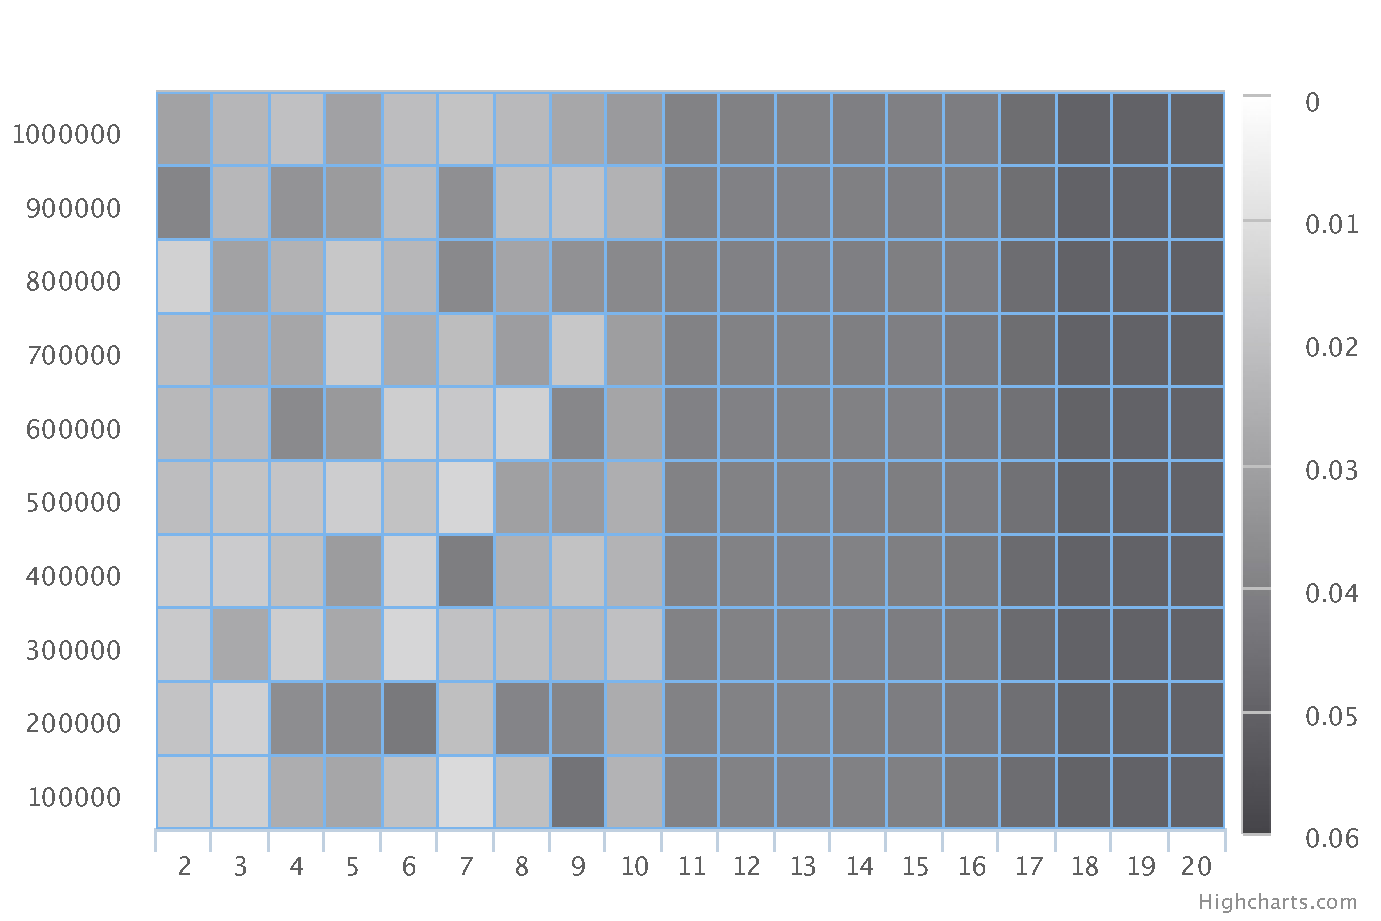
\includegraphics[width=1.0\textwidth]{time-zadig}
    \caption{Temps d'exécution du programme avec le texte de Zadig}
    \label{fig:time-zadig}
\end{figure}

On remarque, surtout avec Don Quixote \ref{fig:time-don-quixote}
\ref{fig:time-don-quixote-plot}, que $k=2$ estun cas où le temps d'exécution
est très élevé. De plus, la génération de donnée a été arrêté pour le cas $k=1$
car il prennait beaucoup trop de temps. A part ces cas particuliers, le temps
d'exécution est à peu près croissante linéairement en fonction de $k$. \\

On remarque également, avec les texte de Madame de Bovary \ref{fig:time-madame}
et de Zadig \ref{fig:time-zadig}, que les temps deviennent constants quand $m$
varie après un certain $k$ ($k=11$ pour Zadig et $k=15$ pour Madame de Bovary). \\

Si le temps d'exécution n'est pas constant par rapport à $m$, on remarque
qu'avec le cas de Don Quixote \ref{fig:time-don-quixote-plot-m} qu'il croit en
logarithme en fonction de $m$. \\

\subsubsection{Nombre d'appel \emph{count3}}

\begin{figure}[ht]
    \centering
    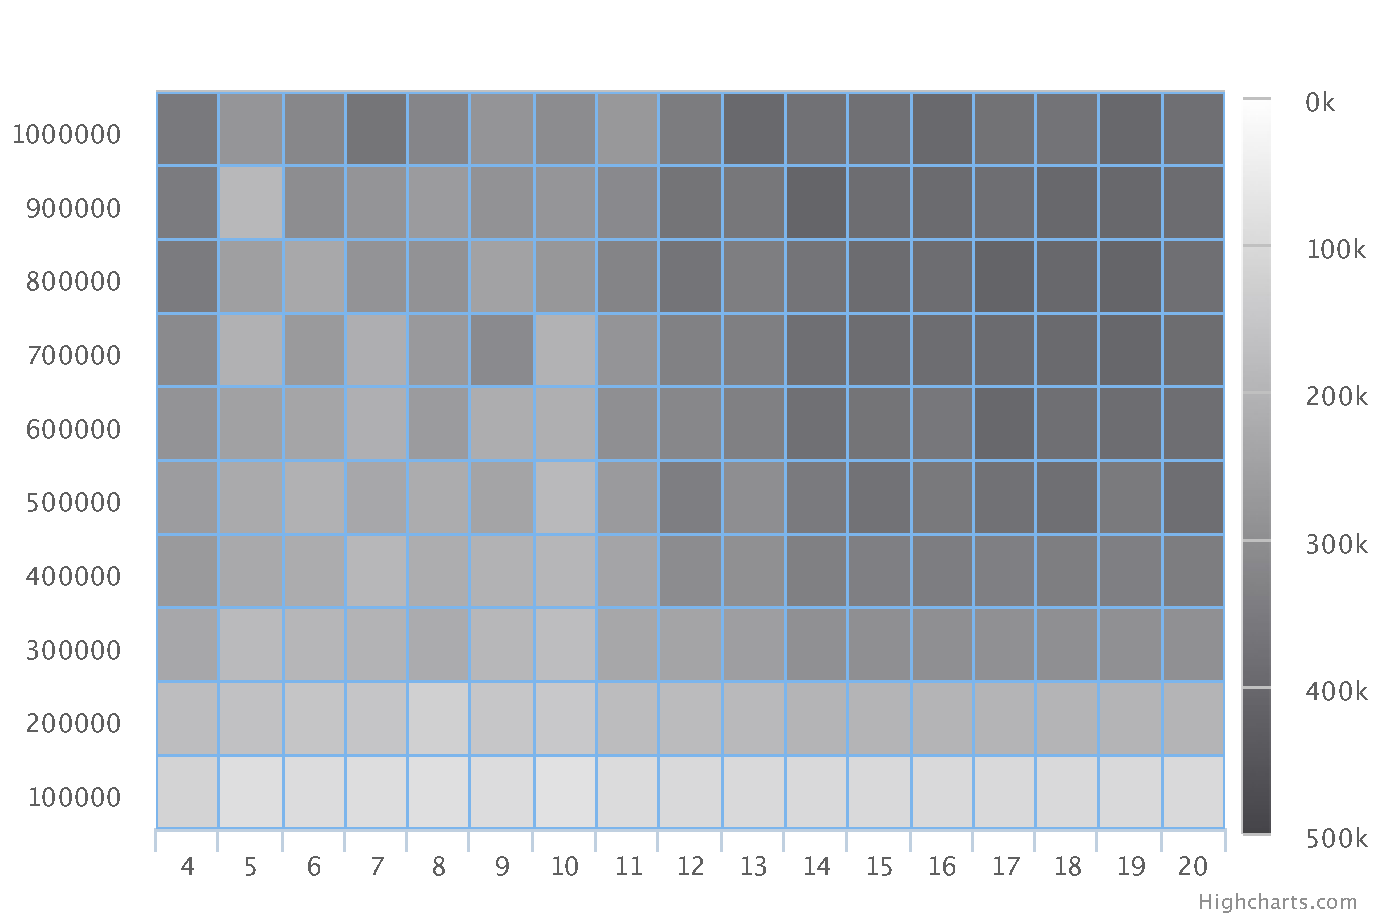
\includegraphics[width=1.0\textwidth]{count-don-quixote}
    \caption{\emph{count3} avec le texte de Don Quixote}
    \label{fig:count-don-quixote}
\end{figure}

\begin{figure}[ht]
    \centering
    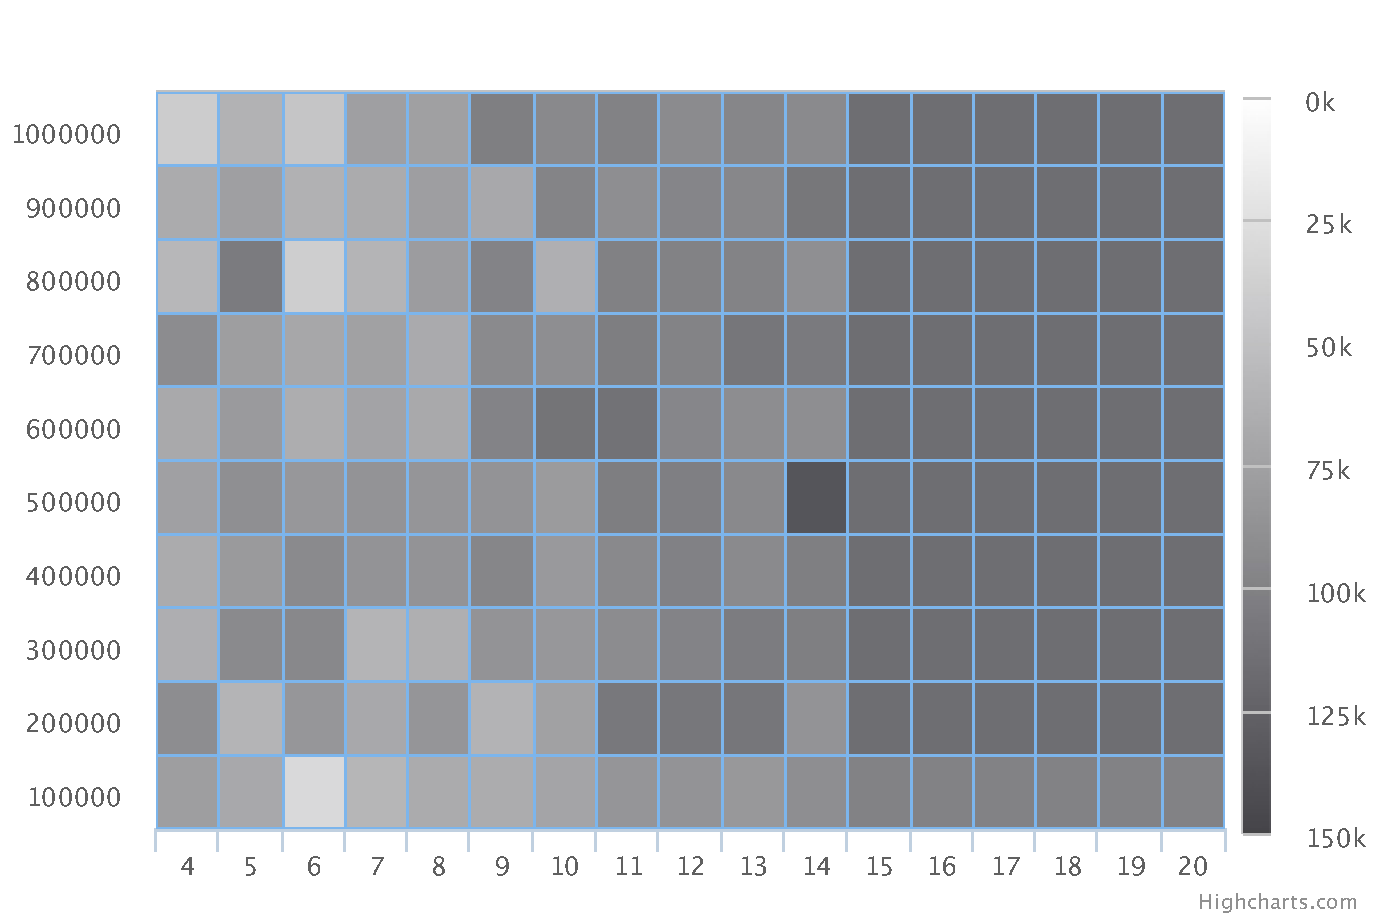
\includegraphics[width=1.0\textwidth]{count-madame}
    \caption{\emph{count3} avec le texte de Madame de Bovary}
    \label{fig:count-madame}
\end{figure}

\begin{figure}[ht]
    \centering
    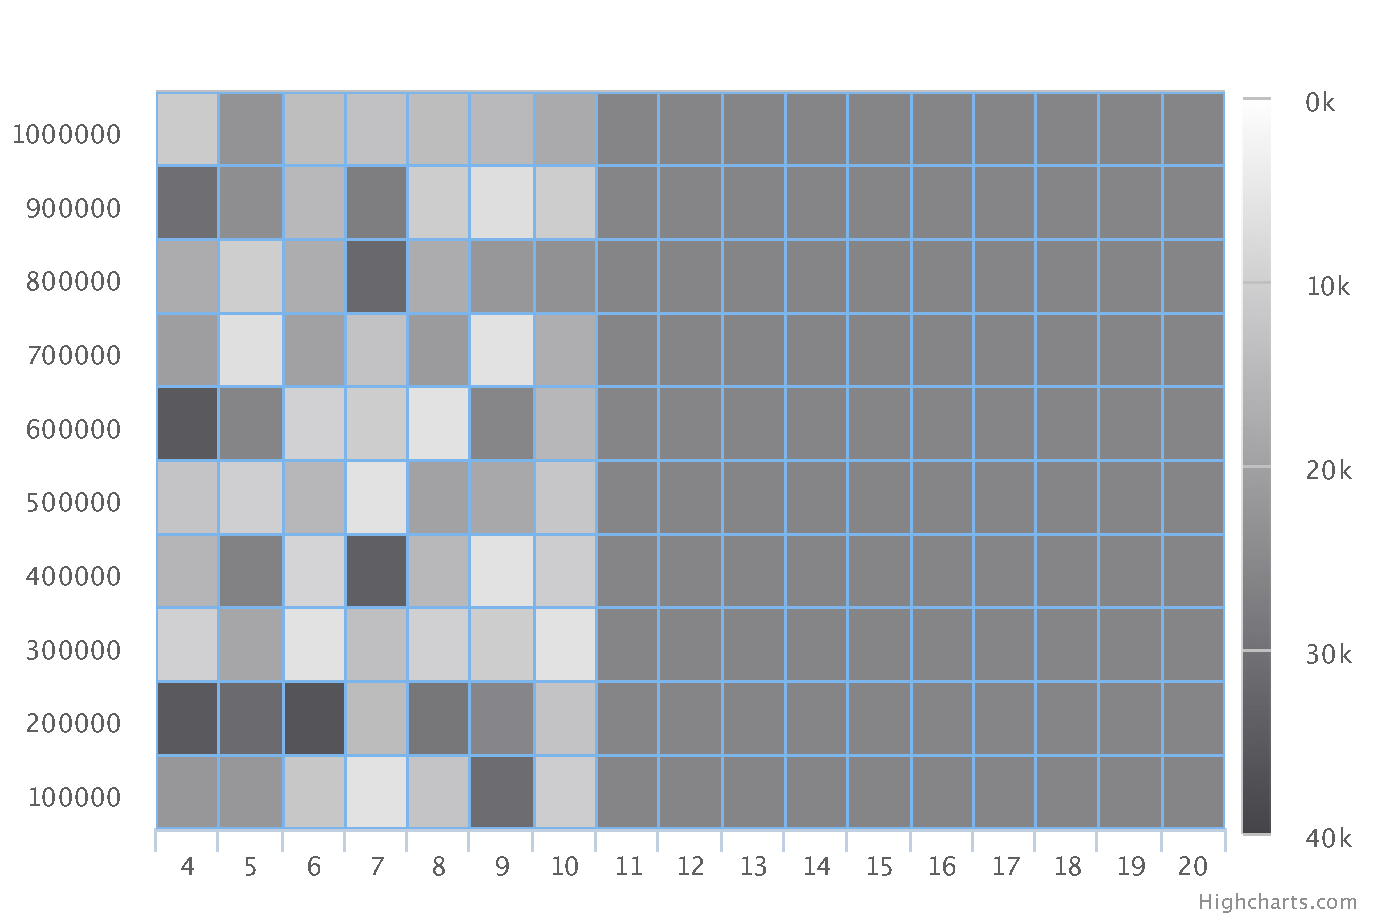
\includegraphics[width=1.0\textwidth]{count-zadig}
    \caption{\emph{count3} avec le texte de Zadig}
    \label{fig:count-zadig}
\end{figure}

On remarque avec Madame de Bovary \ref{fig:count-madame} et Zadig
\ref{fig:count-zadig} que \emph{count3} devient constant à partir d'un certain
$k$. Cette valeur de $k$ est la même qui rend le temps d'exécution constant par
rapport à $m$ ($k=11$ pour Zadig et $k=15$ pour Madame de Bovary).

On voit avec Don Quixote \ref{fig:count-don-quixote} que $k$ n'a pas une très
grande influence sur la valeur de \emph{count3}. En effet celle-ci croît
linéairement en fonction de $m$. En fonction de $k$, sa valeur chute très
rapidement au début \footnote{k=2 et k=3 ont était retiré de la dataviz car ils
avaient une valeur trop importante et rendaient le reste du graphique
illisible} puis croit légèrement pour se stabiliser à une valeur fixe. \\

\end{document}
